% To compile a table to a standalone pdf:
% pdflatex savetable.tex
% pdfcrop savetable.pdf
\documentclass{book}
\usepackage[a4paper,top=2cm,bottom=2cm,left=2cm,right=2cm,marginparwidth=1.75cm]{geometry}
\usepackage[dvipsnames]{xcolor}
\usepackage{tabularray}
\UseTblrLibrary{varwidth}
\usepackage{enumitem}
\usepackage{tikz}
\usetikzlibrary{shapes.geometric, arrows, positioning, fit}
\NewTblrEnviron{scenery}
\SetTblrInner[scenery]{
	hlines, vlines,
	% rowsep=1.5pt,
	row{1} = {bg=black, fg=white, font=\bfseries},
	column{1} = {font=\bfseries},
	measure=vbox, stretch=-1
}
\pagestyle{empty}
\begin{document}
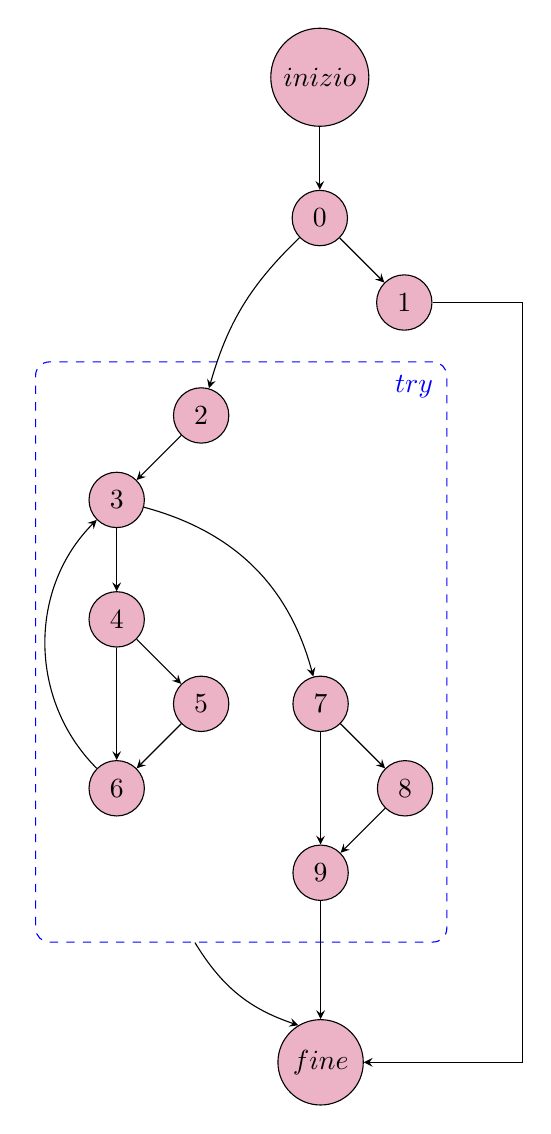
\begin{tikzpicture}[
    node/.style={circle, minimum height=20pt,text centered, draw=black, fill=purple!30},
    try/.style={rectangle, rounded corners=5, dashed, inner sep=12pt, draw=blue},
    node distance=0.8cm,
    arrow/.style={->,>=stealth}
]
\node (start) [node] {$\text{inizio}$};
\node (0) [node, below=of start] {$0$};
\node (1) [node, below right=of 0] {$1$};
\node (2) [node, below left=2cm and 1cm of 0] {$2$};
\node (3) [node, below left=of 2] {$3$};
\node (4) [node, below=of 3] {$4$};
\node (5) [node, below right=of 4] {$5$};
\node (6) [node, below left=of 5] {$6$};
\node (7) [node, right=of 5] {$7$};
\node (8) [node, below right=of 7] {$8$};
\node (9) [node, below left=of 8] {$9$};
\node (try) [try, fit=(2) (3) (4) (5) (6) (7) (8) (9), shift={(-0.25, -0.1)}] {};
\node [anchor=north east, inner sep=5pt, text=blue] at (try.north east) {$\text{try}$};
\node (end) [node, below=1.5cm of 9] {$\text{fine}$};
\draw[arrow] (start) -- (0);
\draw[arrow] (0) -- (1);
\draw[arrow] (0) to [bend right=15] (2);
\draw[arrow] (2) -- (3);
\draw[arrow] (3) -- (4);
\draw[arrow] (4) -- (5);
\draw[arrow] (4) -- (6);
\draw[arrow] (5) -- (6);
\draw[arrow] (6) to [bend left=45] (3);
\draw[arrow] (3) to [bend left] (7);
\draw[arrow] (7) -- (8);
\draw[arrow] (7) -- (9);
\draw[arrow] (8) -- (9);
\draw[arrow] (9) -- (end);
\draw[arrow] (1) -- ++(1.5, 0) |- (end);
\draw[arrow] (try) to [bend right=20] (end) {};
\end{tikzpicture}

\end{document}
